\documentclass[11pt,a4paper]{article}

% -- Encodage et langue --
\usepackage[utf8]{inputenc}
\usepackage[T1]{fontenc}
\usepackage[french]{babel}
\frenchsetup{SmallCapsFigTabCaptions=false}

% -- Mise en page --
\usepackage[margin=2.5cm]{geometry}
\usepackage{setspace}
\onehalfspacing

% -- Packages scientifiques --
\usepackage{amsmath,amssymb}
\usepackage{graphicx}
\usepackage{booktabs}
\usepackage{longtable}
\usepackage{multirow}
\usepackage{xcolor}
\usepackage{placeins}
\usepackage{lineno}
\usepackage{hyperref}
\hypersetup{
    colorlinks=true,
    linkcolor=blue!60!black,
    citecolor=green!50!black,
    urlcolor=blue!70!black
}
\usepackage{cleveref}

% -- Bibliographie --
\usepackage[numbers,sort&compress]{natbib}

% -- Commandes personnalisees --
\newcommand{\todo}[1]{\textcolor{red}{\textbf{[TODO: #1]}}}
\newcommand{\mtb}{\textit{Mycobacterium tuberculosis}}
\newcommand{\spdi}[1]{\texttt{#1}}
\newcommand{\lignee}[1]{\textsf{#1}}
\newcommand{\ang}{\text{\AA}}

\title{L'interrogation domaine par domaine résout Rv2516c, une protéine non étudiée de \mtb{},
  en un domaine de type ferredoxine, une hélice-tour-hélice ailée de la famille AlpA/excisionase,
  et un feuillet $\beta$ de type immunoglobuline}

\author{Christophe Guyeux$^{1,*}$\\[6pt]
  \parbox{\textwidth}{\centering\small
    $^{1}$Institut Femto-ST, UMR 6174 CNRS,\\
    Universit\'e Marie et Louis Pasteur, Besan\c{c}on, France\\[3pt]
    $^{*}$Auteur correspondant~: \texttt{christophe.guyeux@univ-fcomte.fr}
  }
}

\date{}

% ===========================================================
\begin{document}
\linenumbers
\maketitle

\begin{abstract}
\noindent
Une part substantielle du protéome de \mtb{} reste fonctionnellement non caractérisée, et
rechercher une protéine dark pleine longueur qui combine plusieurs domaines indépendants peut
diluer un signal d'homologie distante réel en dessous du seuil de détection. Nous résolvons ici
Rv2516c, une protéine conservée hypothétique de 267 résidus jamais étudiée dans la littérature sur
\mtb{}, en interrogeant séparément chacune de ses unités structurales. La segmentation par carte de
contacts des modèles AlphaFold et ESMFold délimite trois unités~: un domaine N-terminal de type
ferredoxine (résidus 1--87, Pfam DUF8830), une hélice-tour-hélice ailée centrale de la famille
AlpA/excisionase (résidus 88--147), et un feuillet $\beta$ C-terminal de type immunoglobuline
(résidus 178--267) de fonction non assignée. La recherche profil--profil (HHpred) sur la seule
unité centrale identifie la famille AlpA/excisionase à $E=1,3\times10^{-10}$, un gain de plus de
4\,500~fois en valeur $E$ par rapport à la même recherche sur la protéine entière, renversant deux
hypothèses antérieures plus faibles portant sur la protéine entière (repli de type protéine
ribosomale S6, région isolée de facteur sigma). Rv2516c est co-transcrite avec Rv2517c dans une
cassette génomique ancienne et domestiquée, aux côtés d'une paire toxine--antitoxine validée~; la
réanalyse de données RNA-seq la montre induite sous traitement antibiotique comme une réponse de
stress générale, et non la réponse aux dommages de l'ADN (SOS) que son seul contexte génomique
avait suggérée. Quatre lignes de preuve indépendantes, homologie, charge de surface exposée,
conservation inter-genre, et géométrie de contact à résolution atomique dans un modèle de
co-repliement protéine--ADN, convergent sur les mêmes résidus basiques (Arg111, Arg113, His115,
Arg118) comme surface candidate de liaison à l'ADN, bien qu'aucune ne soit significative isolément,
qu'aucun motif opérateur n'ait pu être trouvé à proximité, et qu'un test d'auto-association du
domaine soit resté non informatif. Rv2516c n'est pas essentielle au sens strict de la mutagenèse
par transposon, puisque le module hélice-tour-hélice ne porte aucun site d'insertion de
transposon, mais elle est fortement vulnérable à l'interférence CRISPR (indice de vulnérabilité
$-9,91$, dont la fiabilité a été confirmée indépendamment), restreinte au genre
\textit{Mycobacterium} et à ses plus proches parents, et entièrement non étudiée. Nous proposons
l'interrogation domaine par domaine comme stratégie générale pour les protéines dark
multi-domaines, et avançons le module hélice-tour-hélice de Rv2516c comme élément candidat, bien
que non prouvé, de liaison à l'ADN, intégré dans une cassette génomique dérivée d'un élément
mobile.
\end{abstract}

\textbf{Mots-cl\'es~:} \textit{Mycobacterium tuberculosis}, protéome dark, Rv2516c, AlpA/excisionase,
recherche d'homologie domaine par domaine, hélice-tour-hélice, cible thérapeutique

\section{Introduction}

Vingt-huit ans après l'achèvement du génome de \mtb{} H37Rv \citep{cole1998genome}, une grande
partie de son protéome est encore annotée comme « conservée hypothétique » ou ne porte qu'un
domaine de fonction inconnue. La mutagenèse par transposon à l'échelle du génome
\citep{dejesus2017essentiality} et les cribles de vulnérabilité par interférence CRISPR
\citep{bosch2021vulnerability} montrent que certaines de ces protéines dark sont essentielles à la
croissance et hautement sensibles à une inhibition partielle, le profil recherché pour une cible
thérapeutique, et pourtant restent entièrement négligées parce qu'on ne sait rien de leur fonction
moléculaire. Un obstacle supplémentaire est méthodologique plutôt que biologique~: quand une
protéine dark combine en réalité plusieurs domaines structuraux indépendants, la rechercher comme
une seule requête pleine longueur dilue tout signal d'homologie distante qu'un domaine isolé
pourrait porter, parce que le score est calculé, et la significativité statistique évaluée, sur la
séquence ou la structure entière à la fois.

Rv2516c est une protéine de 267 résidus de cette classe. Elle ne porte aucun domaine nommé dans le
balayage Pfam au seuil de gathering standard, sa fiche UniProt (I6YDM0) n'offre qu'une annotation
générique de « protéine à domaine hélice-tour-hélice », et un balayage exhaustif de la littérature
ne la trouve mentionnée qu'en passant, à l'intérieur de listes de gènes, jamais comme sujet d'une
étude. Elle se situe immédiatement en amont de Rv2517c, un gène de 83 résidus avec lequel elle se
chevauche sur quatre paires de bases sur le même brin, lui-même adjacent à une paire
toxine--antitoxine validée expérimentalement, Rv2514c--Rv2515c \citep{tandon2019ta}. Rv2516c est
essentielle par mutagenèse par transposon \citep{dejesus2017essentiality}, fortement vulnérable à
l'inhibition par interférence CRISPR \citep{bosch2021vulnerability}, détectée par spectrométrie de
masse, et quasi invariante à travers les isolats cliniques, autant d'éléments qui en font une
cible candidate abordable et jamais étudiée pour elle-même.

Trois hypothèses successives sur le repli entier de la protéine Rv2516c, un repli de type protéine
ribosomale S6, une région 4 isolée de facteur sigma, et un régulateur de la famille Lrp/AsnC, ont
chacune semblé défendables examinées isolément et ont chacune été renversées par un test plus
ciblé. En tirant les leçons de cette succession de faux départs, nous avons interrogé Rv2516c
domaine par domaine plutôt que comme une requête unique. Segmenter la protéine par sa carte de
contacts internes résout trois unités structurales indépendantes, et rechercher chacune séparément,
plutôt que la séquence entière de 267 résidus, élève la significativité du signal le plus fort de
plus de trois ordres de grandeur et identifie une homologie confiante, jusque-là non détectée. Nous
rapportons ici cette architecture domaine par domaine, le contexte génomique et transcriptionnel du
gène, et un argument convergent, multi-méthodes mais encore non prouvé, en faveur d'un site
candidat de liaison à l'ADN sur le domaine hélice-tour-hélice résolu.

\section{Matériel et Méthodes}

\paragraph{Séquence, modèle de structure et délimitation des domaines.} La séquence protéique de
Rv2516c (UniProt I6YDM0, NP\_217032.2, 267 aa, coordonnées H37Rv 2\,832\,710--2\,833\,513 sur le
brin moins) a été prise dans le génome de référence H37Rv (NC\_000962.3) \citep{cole1998genome}.
Les modèles de structure ont été obtenus depuis l'AlphaFold Protein Structure Database (version v6)
\citep{jumper2021alphafold,varadi2022afdb} et depuis ESMFold. Les unités structurales indépendantes
ont été délimitées en balayant la carte de contacts inter-résidus des deux modèles à la recherche
d'une fenêtre présentant nettement moins de contacts avec le reste de la chaîne qu'avec elle-même,
un critère appliqué à l'aveugle de toute hypothèse de domaine préalable~; les deux modèles ont
rendu des frontières concordantes. La prédiction de transmembranaire et de localisation
subcellulaire a utilisé DeepTMHMM \citep{hallgren2022deeptmhmm}.

\paragraph{Recherche d'homologie structurale et par profil.} Chaque unité, et la protéine entière,
a été recherchée indépendamment contre les bases PDB\_mmCIF70, Pfam-A et SCOPe70 telles que
distribuées par le MPI Bioinformatics Toolkit au moment de la soumission (2026-07-31) par HHpred en
profil--profil \citep{zimmermann2018hhpred}, contre une base Foldseek construite localement des
structures AlphaFold/Swiss-Prot et PDB (build Foldseek 427df8a~; base structurale PDB téléchargée
le 2025-07-25) par Foldseek \citep{vankempen2024foldseek}, et contre la bibliothèque de profils
Pfam-A distribuée par InterPro \citep{paysanlafosse2023interpro} par \texttt{hmmscan}, au seuil de
gathering (calculé le 2026-06-01) et, pour les correspondances sous ce seuil, en dessous (calculé
le 2026-07-31). L'assignation de famille exigeait une convergence entre au moins deux de ces trois
méthodes~; une correspondance isolée d'une seule méthode a été traitée comme suggestive, jamais
comme une assignation.

\paragraph{Essentialité, vulnérabilité et conservation de population.} Les comptes d'insertion de
transposon par site dinucléotidique TA et l'appel d'essentialité ont été pris dans le jeu de
données TnSeq Himar1 publié \citep{dejesus2017essentiality}~; les sites ont été projetés sur les
trois unités structurales pour tester si la couverture par transposon, et donc l'appel
d'essentialité lui-même, s'étend à chaque unité. L'indice de vulnérabilité CRISPRi et son
intervalle de confiance ont été pris chez \citet{bosch2021vulnerability}~; sa fiabilité a été
évaluée indépendamment contre une ressource cataloguant, à l'échelle du génome, le nombre de guides
et la force du guide individuel le plus fort sous-tendant l'estimation de vulnérabilité de chaque
gène, contre la distribution de ces deux quantités sur l'ensemble des gènes classés druggables
($\text{VI}\leq-6,0$, $n=500$). La variation intra-complexe a été tirée d'une base de données locale
de 145\,209 génomes MTBC (format SPDI, référencés sur H37Rv)~; la conservation inter-genre a
utilisé \texttt{tblastn} (BLAST+ 2.15.0) contre les génomes de six mycobactéries non tuberculeuses
connues pour porter un orthologue de Rv2516c, relancé avec des alignements pairés complets (pas
seulement des résumés d'identité) afin que la conservation par résidu, et pas seulement l'identité
sur la protéine entière, puisse être calculée~; trois des six génomes (\textit{M.\ avium},
\textit{M.\ bouchedurhonense}, \textit{M.\ timonense}) se sont révélés partager un profil
d'identité par position identique, cohérent avec leur appartenance au complexe \textit{M.\ avium},
et ont été traités comme une seule observation phylogénétiquement indépendante afin d'éviter la
pseudo-réplication, laissant quatre lignées indépendantes.

\paragraph{Contexte génomique, synténie et réseau régulateur.} La fenêtre de six gènes flanquant
Rv2516c (Rv2512c--Rv2518c) a été caractérisée pour des signatures de transfert horizontal (sites
d'attachement flanquants, gènes d'ARNt, contenu en GC calibré contre la distribution au niveau
gène à l'échelle du génome) et pour la co-expression avec son voisin immédiat Rv2517c et avec la
paire toxine--antitoxine validée Rv2514c--Rv2515c \citep{tandon2019ta}, en utilisant deux
compendiums d'expression publiés indépendants. Les associations régulatrices ont été prises dans le
réseau de liaison des facteurs de transcription de \mtb{} à l'échelle du génome
\citep{minch2015network} et dans les données d'association protéique récupérées via STRING v12.0
\citep{szklarczyk2023string}.

\paragraph{Réponse transcriptionnelle sous stress antibiotique.} Des données RNA-seq déposées
publiquement, couvrant \mtb{} exposée à la moxifloxacine et, séparément, à neuf antibiotiques de
six classes mécanistiques distinctes, ont été réanalysées pour Rv2516c, Rv2517c et le marqueur
canonique de la réponse SOS \textit{recA}. L'induction de Rv2516c sous moxifloxacine a été comparée
à celle de \textit{recA} et \textit{dnaE2} (témoins de la réponse SOS), et sa réponse à travers des
antibiotiques mécanistiquement distincts (moxifloxacine, capréomycine, kanamycine) a été corrélée à
celle de \textit{recA} pour tester si l'induction suit spécifiquement les dommages à l'ADN ou le
stress antibiotique en général \citep{iacobino2021moxifloxacin}.

\paragraph{Charge de surface et cartographie de la conservation inter-genre.} L'accessibilité au
solvant relative par résidu a été calculée sur le modèle AlphaFold par l'algorithme de
Shrake--Rupley \citep{shrake1973sasa}, normalisée par l'accessibilité au solvant maximale autorisée
de chaque type de résidu \citep{tien2013maxasa}. La fraction de résidus basiques exposés a été
comparée entre l'hélice de reconnaissance candidate (résidus 111--121), l'hélice adjacente, l'unité
hélice-tour-hélice entière, l'unité de type ferredoxine (témoin de spécificité), et la protéine
entière.

\paragraph{Co-repliement Boltz-2, témoin mutant et analyse des contacts d'interface.} Boltz-2,
version 2.2.1, \citep{wohlwend2025boltz2} a été exécuté localement (inférence CPU) pour prédire des
complexes entre l'unité hélice-tour-hélice et un duplex d'ADN double brin de 22 pb dérivé d'un
opérateur co-cristallisé d'un régulateur actinobactérien validé de liaison à l'ADN (BldC, PDB
6AMA), utilisé tout au long de l'étude comme ligand témoin positif~; un témoin de spécificité a
substitué l'unité de type ferredoxine au même duplex, et un témoin négatif a muté trois résidus
basiques candidats de l'hélice de reconnaissance en alanine (R113A/H115A/R118A) avant de relancer
la prédiction. Au-delà du pTM d'interface agrégé et de l'erreur alignée prédite, les distances
atome par atome entre chaque atome protéique et chaque atome d'ADN ont été calculées directement à
partir des coordonnées mmCIF prédites (en utilisant les identifiants d'auteur des chaînes et
résidus, non les identifiants internes) pour les prédictions sauvage et mutante, afin que la
réponse géométrique du modèle à la mutation puisse être évaluée indépendamment du score agrégé.
L'auto-association de l'unité hélice-tour-hélice a été testée de la même façon, en homodimère apo,
contre un témoin négatif de spécificité (l'unité de type ferredoxine) et un témoin positif (BldC
apo), les trois sous des réglages identiques (CPU, échantillon de diffusion unique).

\paragraph{Recherche de motif opérateur.} Les quatre régions intergéniques flanquant la fenêtre
Rv2512c--Rv2518c ont été balayées à la recherche du meilleur score de répétition inversée puis,
indépendamment, de répétition directe (bras de 6 à 12 pb, espaceur de 0 à 8 pb, jusqu'à deux
disparités par bras), chacune évaluée contre deux modèles nuls~: des permutations à dinucléotides
mélangés de la même région, et un échantillon apparié de régions intergéniques réelles de H37Rv de
longueur comparable. Une région n'était retenue comme candidate que si elle dépassait les deux
distributions nulles~; le seuil de significativité a été corrigé par Bonferroni pour les deux
formes de motif testées sur les quatre régions (huit tests, $\alpha=0,05/8$), fixé avant que l'une
ou l'autre recherche ne soit lancée.

\paragraph{Co-occurrence phylogénétique.} Le recouvrement entre les ensembles de mycobactéries non
tuberculeuses portant un orthologue de Rv2516c et un orthologue de Rv2517c a été évalué par
l'indice de Jaccard et comparé à deux modèles nuls~: des paires de gènes à l'échelle du génome
appariées uniquement sur la rareté de leur ensemble porteur, et, plus strictement, des paires de
gènes voisins à l'échelle du génome appariées en plus sur la rareté.

\paragraph{Détection de poches et druggabilité.} Le modèle AlphaFold apo a été évalué pour la
druggabilité de ses poches avec fpocket 4.2.3, calibré contre une population appariée de 150
structures d'enzymes prouvées et 150 protéines non catalytiques traitées par le même pipeline.

\section{Résultats}

\subsection{Rv2516c est une protéine réelle, non étudiée, dont l'essentialité est restreinte à un
domaine tandis que sa vulnérabilité CRISPRi est confirmée fiable indépendamment}

Rv2516c est un authentique produit de gène~: elle est détectée par spectrométrie de masse dans 10
des 16 jeux protéomiques agrégés dans PaxDb \citep{huang2023paxdb}, ne porte que neuf sites
polymorphes sur 145\,209 génomes MTBC (deux synonymes, sept faux-sens, aucun variant non-sens ou de
décalage du cadre de lecture), et est restreinte au genre \textit{Mycobacterium} et à ses plus
proches parents (6 des 53 mycobactéries non tuberculeuses échantillonnées, 1 des 4 membres du
complexe associé à \mtb{} hors du genre). Un balayage exhaustif de la littérature sur environ
330\,000 résumés tuberculose, utilisant chaque alias connu du locus, ne trouve pas une seule
publication qui traite Rv2516c comme sujet~; les sept publications où le locus tag apparaît ne le
citent qu'à l'intérieur de listes de gènes supplémentaires.

Le gène est essentiel, mais pas uniformément sur toute sa longueur. Sur les quatorze sites
dinucléotidiques TA disponibles à la mutagenèse par transposon Himar1 dans Rv2516c, cinq sont
appelés essentiels et neuf non essentiels \citep{dejesus2017essentiality}, le motif que ce même
crible classe comme « Essential-Domain » plutôt qu'uniformément essentiel. Projetés sur les trois
unités structurales résolues plus bas (Section~3.2), les cinq sites essentiels se regroupent
entièrement dans l'unité N-terminale de type ferredoxine, tandis que l'unité hélice-tour-hélice
centrale ne porte \emph{aucun} site TA du tout et est donc structuralement invisible à ce test, non
confirmée non essentielle par lui. L'essentialité du module hélice-tour-hélice, l'unité centrale de
l'hypothèse de liaison à l'ADN développée plus bas, est donc inconnue plutôt qu'établie, et
l'attribution de l'essentialité à l'unité de type ferredoxine repose sur une coïncidence de compte
de sites plutôt que sur une preuve directe site par site.

À l'inverse, l'indice de vulnérabilité à l'interférence CRISPR du gène, $-9,91$ (IC 95~\% $-11,01$ à
$-8,79$) \citep{bosch2021vulnerability}, n'est pas un artefact d'un panel de guides ténu. Vérifié
contre une ressource qui répertorie, pour chaque gène du crible, le nombre de guides contributeurs
et la force du guide unique le plus fort, Rv2516c est soutenue par 51 guides (45,6e percentile
parmi les gènes druggables) avec une force de guide maximale de 0,91 (27,8e percentile, au-dessus
du seuil de fiabilité conventionnel de 0,8). Ceci importe parce qu'un indice de vulnérabilité
extrême calculé à partir d'un panel de guides faible n'est pas fiable, et une force de guide
maximale sous 0,8 est un marqueur reconnu d'une telle non-fiabilité dans ce crible~; les gènes en
bas de cette distribution peuvent porter une estimation de vulnérabilité extrême mais en définitive
non soutenue. Le panel de guides de Rv2516c, bien qu'en dessous de la force médiane des gènes
druggables (0,952), franchit cette barre de fiabilité, si bien que sa vulnérabilité est rapportée
telle que mesurée, et non extrapolée.

\subsection{L'interrogation domaine par domaine résout trois unités structurales indépendantes et
renverse deux hypothèses antérieures portant sur la protéine entière}

La segmentation par carte de contacts des modèles AlphaFold et ESMFold converge indépendamment vers
la même architecture à trois unités~: une unité N-terminale A (résidus 1--87), une unité centrale B
(résidus 88--147), un court lien (résidus 148--177), et une unité C-terminale C (résidus 178--267)
(\Cref{fig:architecture}a).

\begin{figure}[htbp]
\centering
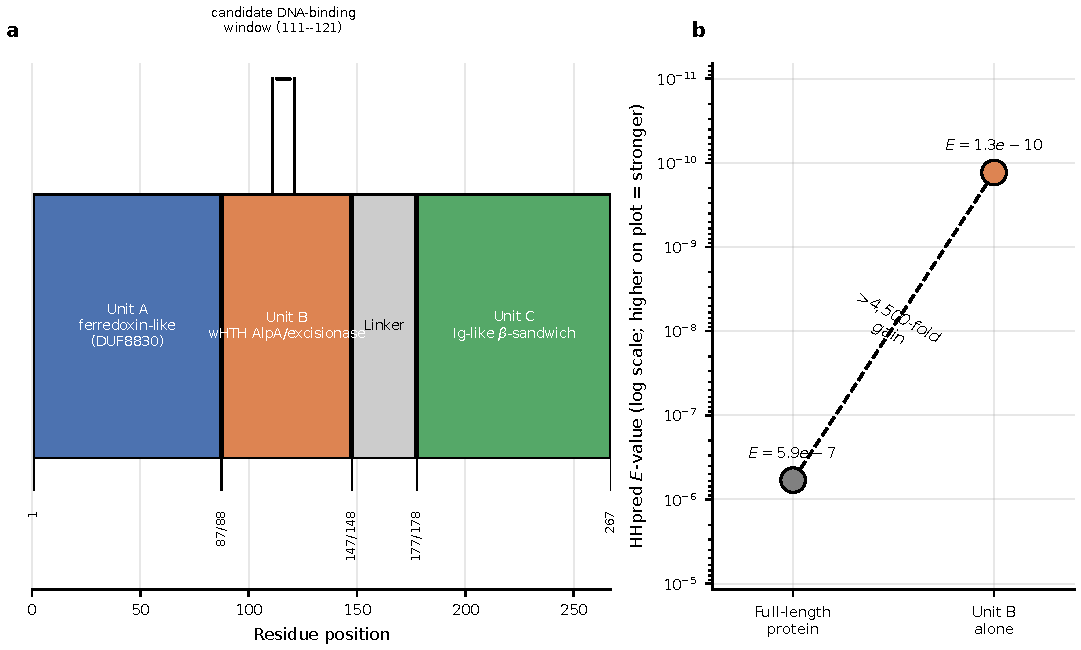
\includegraphics[width=\linewidth]{figures/figure1_architecture.pdf}
\caption{L'interrogation domaine par domaine résout Rv2516c. \textbf{(a)} Architecture linéaire des
267 résidus, délimitée par segmentation en carte de contacts des modèles AlphaFold et ESMFold~: un
domaine N-terminal de type ferredoxine (unité A, DUF8830), une hélice-tour-hélice ailée centrale de
la famille AlpA/excisionase (unité B), un court lien, et un feuillet $\beta$ C-terminal de type
immunoglobuline (unité C) de fonction non assignée. La fenêtre candidate de liaison à l'ADN
(111--121, \Cref{fig:convergence}) se situe au sein de l'unité B. \textbf{(b)} La recherche
profil--profil (HHpred) sur la seule unité B élève la valeur $E$ de l'assignation
AlpA/excisionase de plus de 4\,500~fois par rapport à la même recherche sur la protéine entière,
renversant deux hypothèses antérieures plus faibles portant sur la protéine entière (repli de type
S6 ribosomal, région isolée de facteur sigma).}
\label{fig:architecture}
\end{figure}

Deux hypothèses portant sur la protéine entière ont précédé cette segmentation et ont chacune été
abandonnées une fois testées directement. La première a lu la meilleure correspondance Foldseek
unique contre la Protein Data Bank complète, des permutants circulaires de la protéine ribosomale
S6, comme une assignation de repli~; une comparaison TM-align ciblée contre trois jeux de référence
nommés (permutants S6 ribosomaux, région 4 de facteur sigma, régulateurs de liaison à l'ADN de la
famille MerR) a montré ensuite que cette correspondance n'était que la plus forte d'un plancher de
bruit inter-classes (score TM de 0,33--0,47 sur les trois familles), pas un signal discriminant. La
seconde hypothèse reposait sur l'unique domaine Pfam montré dans un rapport-résumé (région 4 de
facteur sigma, Sigma70\_r4, résidus 98--121, $E=8,4\times10^{-4}$ indépendante, sous le seuil de
gathering de Pfam)~; la sortie complète de \texttt{hmmscan} contenait en fait douze correspondances
sous le seuil couvrant douze familles distinctes d'hélice-tour-hélice sans famille dominante
unique, si bien qu'« une région isolée de facteur sigma » n'était qu'une candidate parmi d'autres
plutôt qu'une assignation privilégiée. Une troisième hypothèse, un régulateur de la famille
Lrp/AsnC, a été exclue par un test structural contrôlé qui a rendu des scores au plancher de bruit
(0,397 et 0,275) et par l'ordre inversé de ses deux domaines putatifs par rapport à la véritable
architecture Lrp/AsnC.

En tirant les leçons de ce motif, à savoir que chaque signal apparent provenait en réalité de la
requête entière de 267 résidus diluant ce qu'un domaine isolé portait, l'unité B a été soumise à
HHpred seule. Le résultat est la découverte la plus confiante de cette étude~: probabilité
99,28~\%, $E=1,3\times10^{-10}$, assignant l'unité B à la famille AlpA/excisionase/facteur de
directionnalité de recombinaison, contre une probabilité de 98,64~\%, $E=5,9\times10^{-7}$ pour la
même recherche sur la protéine entière, un gain de plus de 4\,500~fois en valeur $E$ du simple fait
d'isoler le domaine. Ni l'hypothèse S6 ribosomale, ni celle de la région 4 de facteur sigma, ni
celle Lrp/AsnC ne survivent à ce résultat. Une réserve s'applique~: \texttt{hmmscan} ne retrouve
jamais le profil AlpA à aucun seuil, sur aucune unité, alors même que HHpred interroge la même
bibliothèque Pfam-A sous-jacente et retourne le profil correspondant (PF11112) à 99,16~\% de
probabilité sur l'unité B~; les profils sont atteignables en principe, et l'écart reflète le régime
de sensibilité séquence-contre-profil plutôt qu'une réfutation de l'assignation.

L'unité A porte indépendamment un second domaine nommé, DUF8830 (domaine de fonction inconnue
8830, Pfam PF31169, probabilité 98,16~\%, $E=1,2\times10^{-4}$, 81 des 87 colonnes alignées), une
famille restreinte aux actinomycètes sans fonction connue, sans structure résolue et sans
appartenance à un clan Pfam. Les deux domaines sont, dans leurs familles respectives, presque
toujours trouvés seuls~: DUF8830 apparaît comme seul domaine annoté chez 863 des 864 membres de la
famille (99,9~\%), et la famille contenant AlpA (qui inclut aussi DUF1233, PyocinActivator et des
membres de type Tn916-Xis) chez 10\,141 des 10\,168 (99,7~\%). Rv2516c fusionne donc deux domaines
qui constituent chacun, dans pratiquement tout autre génome, une protéine complète à eux seuls~;
aucun des 25 partenaires de fusion connus de la famille AlpA ne la combine à un domaine de type
ferredoxine ou immunoglobuline. L'assignation de repli de l'unité C et son assignation
fonctionnelle reposent sur des preuves différentes et aboutissent à des conclusions différentes, et
les deux ne doivent pas être lues comme également incertaines. Le \emph{repli} en feuillet $\beta$
de type immunoglobuline est soutenu par un consensus entre les deux méthodes~: indépendamment chez
Foldseek et chez HHpred, et au sein de HHpred par convergence entre plusieurs familles Pfam
d'immunoglobulines non apparentées, la classe SCOP « tout-bêta », et, notablement, quatre feuillets
$\beta$ synthétiques conçus \emph{de novo} sans aucune histoire évolutive~; des échafaudages
synthétiques idéalisés de ce type figurent parmi les meilleures correspondances précisément parce
qu'ils s'accordent sur la seule topologie nue, ce qui est diagnostique d'une assignation authentique
au niveau du repli plutôt que d'un artefact d'une seule correspondance limite. L'assignation de
\emph{famille et de fonction} est une question séparée, et négative~: la meilleure correspondance à
domaine nommé est elle-même un domaine de fonction inconnue (Pfam DUF8453, $E=6,1\times10^{-3}$),
bien en deçà de la significativité, si bien qu'aucune famille ni fonction moléculaire ne peut être
assignée au-delà du repli lui-même. Cette dissociation, un repli confiant sans fonction assignable,
n'est pas en tension avec la localisation cytoplasmique, non membranaire, prédite pour Rv2516c
\citep{hallgren2022deeptmhmm}, puisque 8 des 16 protéines de H37Rv portant ce même clan Pfam
(CL0159, E-set) sont elles-mêmes cytoplasmiques, la plupart étant de grandes enzymes portant le
repli de type immunoglobuline comme module accessoire, le même arrangement observé ici.

Cette architecture d'ensemble, une hélice-tour-hélice interne flanquée des deux côtés par des
domaines nommés indépendamment, est rare dans le protéome de H37Rv, pas seulement au sein de la
famille AlpA. Sur 212 protéines de H37Rv portant une hélice-tour-hélice du même clan Pfam (5,4~\%
du protéome annoté), un positionnement \emph{interne} (au moins 50 résidus de séquence flanquante
de chaque côté) est appauvri d'un facteur 3,4 par rapport à un modèle nul uniforme (25 observées
contre 84,0 attendues). Seules trois protéines en dehors de Rv2516c combinent une
hélice-tour-hélice interne à flancs longs sans autre domaine Pfam annoté (Rv1830/MerR, Rv0042c,
Rv0737/MarR), et Rv2516c diffère qualitativement des trois~: ses flancs ne sont pas des extensions
non assignées mais deux domaines repliés identifiés indépendamment. Comme vérification contre
l'attribution erronée d'une fonction nouvelle qui appartiendrait en réalité à un paralogue connu,
nous avons confirmé qu'aucun autre locus de H37Rv ne porte à la fois DUF8830, l'hélice-tour-hélice
de la famille AlpA et le repli de type immunoglobuline~; deux loci non apparentés (Rv2310, Rv3750c)
portent déjà le nom « excisionase » dans l'annotation actuelle sans le domaine correspondant
(seulement une correspondance générique HTH\_17), une collision de nommage qu'il vaut la peine de
signaler pour quiconque cherche dans le génome par nom plutôt que par contenu de domaine. Une
recherche Foldseek de chaque unité séparément contre la base AlphaFold/Swiss-Prot n'a rendu aucune
correspondance significative ni suggestive (meilleure $E=1,7\times10^{-2}$, unité A), n'ajoutant
aucune assignation au-delà de ce que les recherches Protein Data Bank et HHpred ci-dessus avaient
déjà établi.

\subsection{La cassette Rv2516c--Rv2517c est une unité génomique ancienne, domestiquée, qui répond
à un stress antibiotique général et non à des dommages à l'ADN}

Rv2516c et Rv2517c se chevauchent sur quatre paires de bases sur le même brin, cohérent avec un
couplage traductionnel, et se situent immédiatement en amont de la paire toxine--antitoxine validée
expérimentalement Rv2514c--Rv2515c \citep{tandon2019ta}, seul élément ancré expérimentalement de la
fenêtre environnante. Ceci situe la cassette dans un voisinage fonctionnel, mais pas, comme une
lecture antérieure de la région le supposait, comme un répresseur commandant une excisionase~; il
s'agit d'un locus toxine--antitoxine avec une paire adjacente, fonctionnellement distincte.

La fenêtre environnante de six gènes ne montre aucune signature d'acquisition horizontale récente~:
aucune séquence frontière attL/attR, aucun gène d'ARNt discriminant à l'un ou l'autre flanc, et un
contenu en GC tout à fait ordinaire pour Rv2516c elle-même une fois comparé à la distribution à
l'échelle du génome (8,2e percentile parmi 3\,899 gènes, bien à l'intérieur de la fourchette
ordinaire plutôt qu'une valeur aberrante). La conservation gène par gène à travers les mycobactéries
non tuberculeuses varie d'un voisin à l'autre, un motif en mosaïque plus cohérent avec un élément
ancien, pleinement intégré, qu'avec un élément récemment acquis et encore mobile. Cohérent avec
cette lecture, une recherche systématique d'un opérateur palindromique en amont de la transposase
IS1081 voisine et en amont de l'opéron Rv2516c--Rv2517c lui-même n'a rendu aucun candidat~: sur les
quatre régions intergéniques, testées contre le double modèle nul décrit en Méthodes, la meilleure
répétition inversée d'aucune région n'a dépassé les deux modèles nuls (le cas le moins extrême
n'atteignait que $p=0,130$ contre le modèle nul de permutation et $p=0,185$ contre le modèle nul
génomique). Une seconde recherche, pré-enregistrée, des mêmes quatre régions pour la forme
symétrique complémentaire, les répétitions directes, a été tout aussi négative à un seuil corrigé
par Bonferroni ($\alpha=0,00625$ sur les huit tests des deux recherches combinées~; la plus petite
valeur $p$ obtenue était 0,277, bien au-dessus même du seuil non corrigé de 0,05). Ensemble, ces
deux résultats négatifs retirent spécifiquement l'hypothèse que Rv2516c active IS1081 par la même
logique de liaison à un opérateur qu'utilisent d'autres régulateurs de la famille AlpA, dont
l'hélice-tour-hélice C-terminale lie un élément d'ADN défini en amont du gène qu'ils contrôlent
\citep{wen2022alpa}, ainsi que l'hypothèse qu'elle autorégule son propre opéron~; ils ne retirent
pas la liaison à l'ADN en général, puisqu'un mode de liaison asymétrique, à un seul demi-site,
reste intestable sans motif consensus de famille ni données d'empreinte, une limite que nous
énonçons plutôt que de la dissimuler.

La cassette porte néanmoins le premier signal fonctionnel directement mesuré de cette étude. La
réanalyse de données RNA-seq publiées montre Rv2516c induite sous traitement à la moxifloxacine
(0,3$\times$ CMI, 24~h), passant de 57 à 138 RPKM (changement log2 de $+1,27$, 93e percentile du
transcriptome), aux côtés de l'induction massive attendue des gènes de la réponse SOS \textit{recA}
et \textit{dnaE2} \citep{iacobino2021moxifloxacin}. Cette induction n'est cependant pas une réponse
aux dommages de l'ADN~: sur un second compendium indépendant couvrant neuf antibiotiques de six
classes mécanistiques distinctes, Rv2516c répond presque à l'identique sous moxifloxacine (91e
percentile), capréomycine (94e) et kanamycine (93e), dont aucune n'endommage directement l'ADN, et
son induction ne corrèle pas avec celle de \textit{recA} à travers les conditions ($r=-0,04$). La
réponse transcriptionnelle de Rv2516c est donc une réponse générale au stress antibiotique, non une
part de la voie SOS que sa proximité génomique avec un locus toxine--antitoxine validé pourrait
suggérer. Cohérent avec une relation fonctionnelle, et non simplement adjacente, Rv2516c et Rv2517c
sont co-exprimées à travers les conditions ($r=+0,409$, 99e percentile de toutes les paires de
gènes), dépassant le plafond de co-expression fixé par la paire toxine--antitoxine validée
elle-même ($r=+0,360$). L'appariement est néanmoins asymétrique~: Rv2517c n'est pas essentielle et
son propre indice de vulnérabilité, $+0,54$ (IC 95~\% $-1,88$ à $+4,58$), traverse zéro,
argumentant contre un hétérodimère obligatoire entre les deux protéines. Cohérent avec cette
asymétrie, STRING ne liste que trois partenaires protéiques pour Rv2516c (Rv2517c, Rv2515c,
Rv2514c), chacun soutenu uniquement par le canal de voisinage génomique (aucune preuve
expérimentale, de base de données ou de fouille de texte), et chacun lui-même annoté comme
hypothétique~; STRING ne contribue donc aucune hypothèse fonctionnelle indépendante ici. Dans le
réseau de facteurs de transcription à l'échelle du génome \citep{minch2015network}, Rv2516c est une
cible, non elle-même annotée comme facteur de transcription, de cinq régulateurs, parmi lesquels
Rv0081, le relais principal du régulon de dormance DosR, plaçant le gène dans un contexte
régulateur de dormance/hypoxie~; ce contexte est néanmoins découplé sous la condition antibiotique
étudiée ici, où les cibles canoniques de DosR \textit{hspX} et Rv2623 s'effondrent tandis que
Rv2516c elle-même monte, montrant que DosR ne gouverne pas la réponse du gène au stress
antibiotique spécifiquement.

\subsection{Quatre lignes de preuve indépendantes, individuellement non significatives, convergent
sur les mêmes résidus basiques du domaine hélice-tour-hélice}

Au-delà de l'homologie au niveau de la famille établie ci-dessus, trois analyses supplémentaires,
méthodologiquement indépendantes, pointent vers les mêmes résidus spécifiques de l'unité B
(\Cref{fig:convergence}).

\begin{figure}[htbp]
\centering
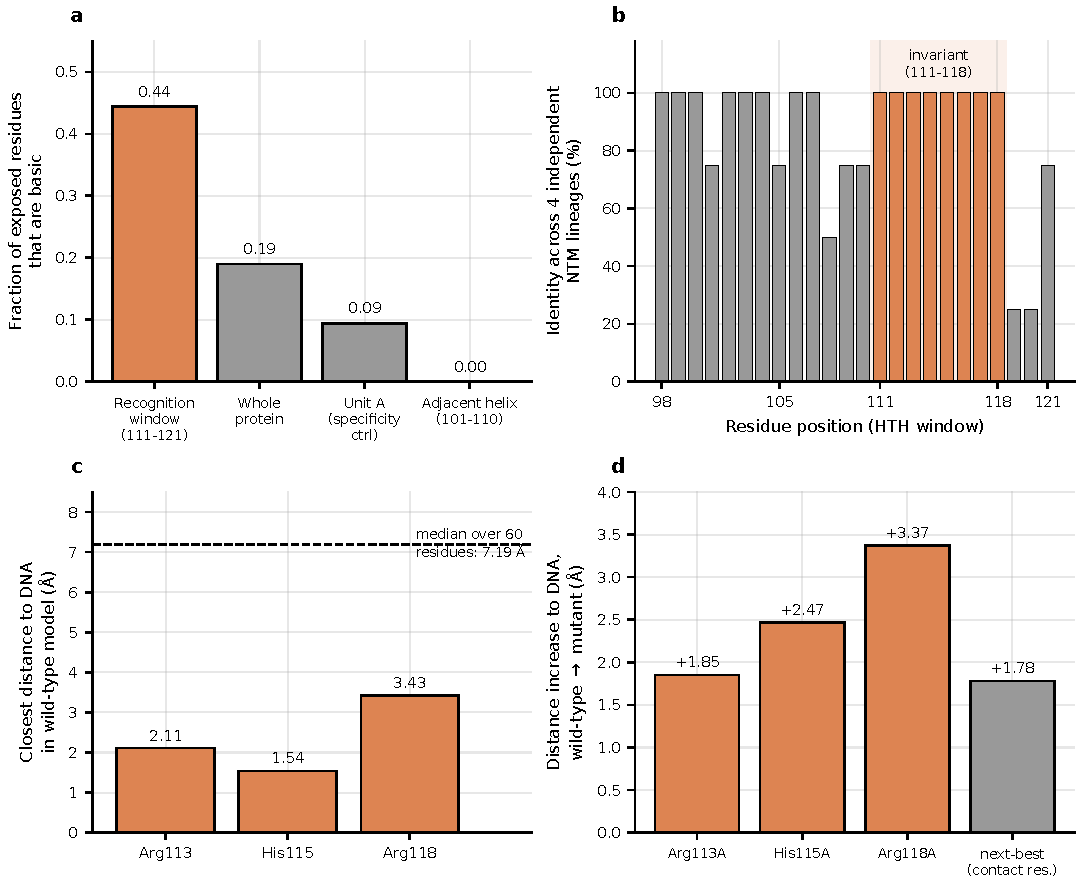
\includegraphics[width=\linewidth]{figures/figure2_convergence.pdf}
\caption{Quatre lignes de preuve indépendantes convergent sur les mêmes résidus basiques du domaine
hélice-tour-hélice. \textbf{(a)} Fraction des résidus exposés qui sont basiques~: la fenêtre de
reconnaissance candidate (111--121) se distingue de la protéine entière, de l'unité A de type
ferredoxine (témoin de spécificité), et de l'hélice immédiatement adjacente. \textbf{(b)} Identité
par position à travers la fenêtre hélice-tour-hélice (98--121) sur quatre lignées mycobactériennes
non tuberculeuses phylogénétiquement indépendantes~; les résidus 111--118 (ombrés) sont invariants
sans exception. \textbf{(c)} Distance la plus proche au duplex d'ADN pour Arg113, His115 et Arg118
dans le modèle de co-repliement Boltz-2 sauvage, comparée à la médiane sur les 60 résidus de
l'unité B. \textbf{(d)} Augmentation de la distance protéine--ADN après substitution en alanine des
trois mêmes résidus (sauvage $\to$ mutant), restreinte aux résidus en contact réel avec l'ADN à
l'état de référence~; la plus grande augmentation suivante parmi les résidus de contact est montrée
pour échelle.}
\label{fig:convergence}
\end{figure}

Premièrement, la charge de surface exposée. Sur l'hélice de reconnaissance putative (résidus
111--121), 0,44 des résidus sont exposés et basiques, contre 0,19 pour la protéine entière, 0,09
pour l'unité A (témoin de spécificité de domaine), et exactement 0,00 pour l'hélice immédiatement
adjacente, qui porte au contraire une charge exposée nette de $-3$. La fenêtre de l'hélice de
reconnaissance elle-même porte une charge exposée nette de $+4$ sans aucun résidu acide exposé. Ce
test repose sur un petit nombre de résidus (quatre positions basiques exposées sur onze dans la
fenêtre) et la séparation azimutale sous-jacente des chaînes latérales basiques et hydrophobes est
une propriété générique de presque toute hélice de surface, non spécifique à la liaison à l'ADN~;
il est rapporté comme une ligne de preuve parmi d'autres, non comme un résultat autonome.

Deuxièmement, la conservation inter-genre. Sur les quatre lignées mycobactériennes non
tuberculeuses phylogénétiquement indépendantes retenues après correction de la pseudo-réplication
du complexe \textit{M.\ avium} (Méthodes), la fenêtre hélice-tour-hélice (résidus 98--121) est
identique à 86,5~\%, contre 62,6~\% pour le reste de la protéine, un excès de 23,9~points qui
survit à la correction (26,3~points non corrigés). Au sein de cette fenêtre, les résidus 111--118
(RQRVHQLR) sont invariants sur les quatre lignées sans exception. Recoupé avec l'analyse de charge
de surface, deux de ces huit positions sont enfouies (Val114, Leu117, cohérent avec une contrainte
d'empilement ordinaire) et six sont exposées (Arg111, Gln112, Arg113, His115, Gln116, Arg118),
parmi lesquelles exactement les trois résidus choisis plus tard, sur des bases structurales seules,
pour le témoin négatif mutant ci-dessous, plus un quatrième.

Troisièmement, la géométrie de contact à résolution atomique issue d'un test direct de
co-repliement protéine--ADN (\Cref{fig:site}). Le score Boltz-2 agrégé est, à lui seul, non
informatif~: l'unité B sauvage et son mutant R113A/H115A/R118A, chacun co-replié avec le même
duplex d'ADN, rendent un pTM d'interface quasi identique (0,890 et 0,889). Lu au niveau des
contacts atomiques plutôt qu'au niveau du score agrégé, le tableau change cependant. Dans la
prédiction sauvage, Arg113, His115 et Arg118 sont authentiquement parmi les contacts les plus
proches de l'ADN dans le modèle entier (2,11, 1,54 et 3,43~\ang{}, contre une médiane de 7,19~\ang{}
sur les 60 résidus de l'unité B~; His115 est le contact le plus proche unique de toute la
structure), pas des résidus périphériques accidentellement proches du duplex. En comparant
atome par atome le sauvage et le mutant, les trois positions mutées montrent les trois plus fortes
augmentations de distance parmi les résidus en contact réel avec l'ADN à l'état de référence
(Arg118 $+3,37$~\ang{}, His115 $+2,47$~\ang{}, Arg113 $+1,85$~\ang{}, contre une augmentation
suivante la plus élevée de $+1,78$~\ang{} parmi les résidus de contact). Quelques résidus déjà
éloignés de l'ADN à l'état de référence ($>9$~\ang{}, près de la frontière C-terminale du fragment
modélisé) se déplacent d'une quantité absolue comparable ou légèrement supérieure (jusqu'à
$+2,10$~\ang{}), cohérent avec un bruit conformationnel ordinaire loin de l'interface plutôt qu'un
effet spécifique du contact avec l'ADN. Restreint aux résidus en contact réel avec l'ADN, le modèle
répond donc correctement à la mutation au niveau de la géométrie locale~; c'est le score agrégé,
calculé sur la structure entière, qui manque de sensibilité pour qu'une perturbation de trois
résidus parmi soixante s'y inscrive. Étalonné contre le témoin positif (BldC lié à son propre
opérateur, le même duplex d'ADN), 27,9~\% des résidus de BldC se situent à moins de 4,5~\ang{} de
l'ADN contre 28,3~\% pour l'unité B, le même ordre de grandeur qu'un régulateur connu pour lier cet
ADN.

\begin{figure}[htbp]
\centering
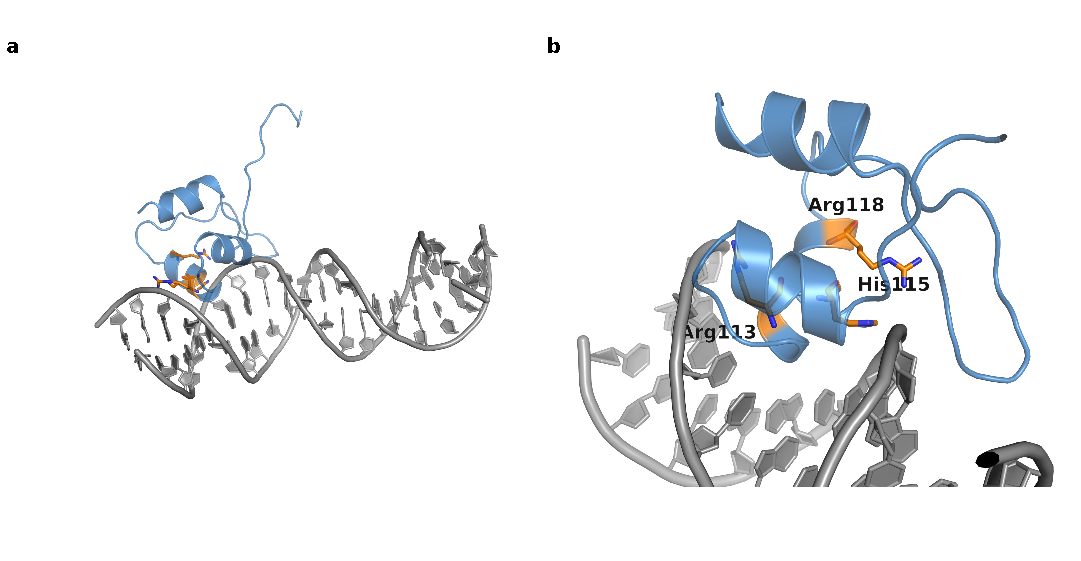
\includegraphics[width=\linewidth]{figures/figure3_site.pdf}
\caption{Contexte structural du site candidat de liaison à l'ADN. \textbf{(a)} Le modèle de
co-repliement Boltz-2 sauvage (J1) place l'unité hélice-tour-hélice (bleu) dans le sillon du duplex
d'ADN (gris)~; les trois résidus de contact candidats sont montrés en bâtonnets (orange).
\textbf{(b)} Gros plan sur l'hélice de reconnaissance, avec Arg113, His115 et Arg118 étiquetés~;
il s'agit du même modèle sous-tendant les distances et la réponse au mutant rapportées en
\Cref{fig:convergence}c,d.}
\label{fig:site}
\end{figure}

Homologie, charge exposée, conservation inter-genre et géométrie de contact atomique, quatre
analyses aux biais méthodologiques indépendants, convergent ainsi sur les mêmes résidus basiques
(Arg111, Arg113, His115, Arg118). Aucune des quatre analyses n'est individuellement significative,
et la convergence est rapportée comme un corps cohérent de preuve circonstancielle en faveur d'une
surface candidate de liaison à l'ADN, non comme une preuve de liaison à l'ADN, encore moins de sa
spécificité de séquence.

\subsection{Les recherches d'opérateur palindromique et à répétition directe sont négatives, et un
test d'auto-association apo manque de puissance pour trancher le mécanisme}

Trois tests supplémentaires ont sondé l'hypothèse de liaison à l'ADN sous des angles différents, et
aucun n'étend la convergence ci-dessus~; chacun restreint un modèle mécanistique spécifique plutôt
que l'hypothèse de liaison à l'ADN en général.

Rv2516c et Rv2517c sont portées par un ensemble identique de génomes mycobactériens non
tuberculeux (6 sur 53, indice de Jaccard 1,000), un fait déjà cité comme preuve d'une unité
génétique étroite mais jamais formellement testé. Contre un modèle nul de paires de gènes appariées
uniquement sur la rareté de l'ensemble porteur (240 gènes, 20\,000 rééchantillonnages),
l'appariement est un authentique cas aberrant (99,9e percentile). Contre un modèle nul apparié plus
strictement, des paires de gènes \emph{voisins} de la même rareté (49 paires comparables à l'échelle
du génome), la concordance parfaite n'est pas unique~: 9 de ces 49 paires (18,4~\%) sont elles-mêmes
à égalité à l'indice de Jaccard 1,000, cohérent avec un effet de bloc régional (gain ou perte
partagés à travers une fenêtre génomique locale) plutôt qu'une signature spécifique à cette paire.
Ce résultat ne touche pas la co-expression fonctionnelle démontrée par RNA-seq ci-dessus
(Section~3.3), qui est une preuve d'une nature différente, mais il retire la co-occurrence
phylogénétique comme argument indépendant en faveur d'un module fonctionnel distinctif.

Les recherches de motif opérateur rapportées en Section~3.3 (répétitions inversées, puis,
pré-enregistrées contre le même seuil corrigé par Bonferroni, répétitions directes) ont été toutes
deux négatives sur les quatre régions intergéniques candidates. Ensemble, elles retirent les
modèles les plus simples d'opérateur palindromique ou en tandem pour cette fenêtre génomique
spécifique, sans exclure un mode de liaison asymétrique, monomérique, que les données et outils
actuels ne peuvent tester.

Enfin, nous avons demandé si l'unité B s'auto-associe en homodimère apo, puisque la dimérisation
est la prémisse structurale d'un modèle d'opérateur palindromique. Le résultat ne tranche pas la
question, pour deux raisons indépendantes et qui se renforcent mutuellement. Sur chaque métrique
(pTM d'interface, erreur alignée prédite inter-chaînes minimale, compte de contacts d'interface),
l'ordre à travers les trois tests d'homodimère apo est l'inverse de ce qu'un test fonctionnel
devrait produire~: le témoin négatif de spécificité (unité A, un domaine sans propension connue à
la liaison à l'ADN) score le plus haut (pTM d'interface 0,873), le test (unité B) score
intermédiaire (0,767), et le témoin positif (BldC apo) score le plus bas (0,564). Premièrement, à
cette gamme de taille (100--200 résidus) et dans ce régime computationnel (CPU, échantillon de
diffusion unique), le test semble replier pratiquement n'importe quel domaine globulaire compact en
un homodimère symétrique plausible et de haute confiance, indépendamment de toute propension
biologique réelle, ce que le score élevé du témoin négatif démontre directement. Deuxièmement, et
indépendamment, le propre score apo de BldC est bien en dessous du score obtenu, dans le même
pipeline, quand BldC est co-repliée avec son opérateur d'ADN (pTM d'interface 0,827, erreur alignée
prédite inter-chaînes minimale 0,64~\ang{}, 113 contacts d'interface, contre 0,564, 4,48~\ang{} et
16 contacts en apo), cohérent avec un mécanisme de dimérisation couplé à l'ADN, plutôt que
constitutif, pour cette famille~; si tel est le cas, un test apo était simplement la mauvaise
expérience pour valider le test sur ce témoin positif. Le propre score de l'unité B ne peut donc
être lu ni comme confirmant l'auto-association, puisqu'un domaine non apparenté score plus haut, ni
comme la réfutant, puisqu'un mécanisme couplé à l'ADN serait par construction invisible à un test
apo. C'est un résultat négatif de méthode, non de biologie, une distinction que nous maintenons de
bout en bout plutôt que de la faire s'effondrer en une lecture confirmatoire ou réfutatoire.

\section{Discussion}

L'interrogation domaine par domaine est le résultat méthodologique qui dépasse ce seul gène.
Rv2516c ressemblait, sous une recherche protéine entière, à une correspondance médiocre et ambiguë
avec plusieurs replis non apparentés tour à tour, la protéine ribosomale S6, une région isolée de
facteur sigma, un régulateur de type Lrp/AsnC, chacune défendable jusqu'à être testée directement
et chacune fausse. Isoler le domaine central et le rechercher seul a élevé le signal disponible le
plus fort de plus de 4\,500~fois en valeur $E$ et a produit la première assignation confiante pour
cette protéine. La leçon se généralise~: une protéine dark qui fusionne en réalité plusieurs
domaines, chacun individuellement caractérisable, peut paraître entièrement opaque, ou pire,
assignable de façon trompeuse à la mauvaise famille, quand elle est traitée comme une requête
unique, parce que le score sur la protéine entière dilue à la fois un signal réel au niveau du
domaine et donne un poids égal à des correspondances faibles et non apparentées ailleurs dans la
séquence.

La convergence de preuves en faveur d'une surface candidate de liaison à l'ADN sur l'unité B,
homologie, charge exposée, conservation inter-genre et géométrie de contact atomique pointant
toutes vers Arg111, Arg113, His115 et Arg118, est, précisément parce qu'elle est désormais
construite à partir de quatre méthodes indépendantes, le point où la discipline anti-survente
importe le plus, et non le moins. Chaque analyse reste individuellement non significative, aucun
test de spécificité de séquence n'a été tenté (le duplex d'ADN utilisé de bout en bout est le
propre opérateur de BldC, pas un site candidat pour Rv2516c), et chaque prédiction structurale
rapportée ici provient d'une méthode de criblage unique (Boltz-2, inférence CPU) plutôt que d'une
structure déterminée expérimentalement ou d'un prédicteur de référence validé. Nous évitons
délibérément d'affirmer que Rv2516c lie l'ADN, encore moins ce qu'elle lie~; le langage approprié,
et celui utilisé tout au long de cette étude, est celui d'un site candidat soutenu par un corps de
preuve convergent mais individuellement non concluant.

Un contexte fonctionnel tentatif, et explicitement non prouvé, mérite d'être énoncé comme une
hypothèse à tester plutôt que comme une conclusion. Le partenaire d'opéron de Rv2516c, Rv2517c, se
situe immédiatement en aval d'une paire toxine--antitoxine validée et est l'un des trois seuls
gènes, aux côtés de la toxine \textit{relK} et de Rv3290c, régulés à la hausse dans un crible qPCR
indépendant de 32~gènes de la réponse à la moxifloxacine, où il est explicitement classé comme gène
lié à la persistance plutôt que comme faisant partie de la réponse SOS
\citep{iacobino2021moxifloxacin}~; ceci est cohérent avec le motif d'induction de stress
antibiotique, et non de dommage à l'ADN, établi directement pour l'opéron par la réanalyse RNA-seq
de la Section~3.3. Avec le contexte régulateur du gène (le relais de dormance DosR Rv0081, un
module de co-expression associé à ArsR) et l'absence générale de Rv2516c de toute littérature
spécifique aux dommages de l'ADN, ceci suggère un rôle lié à la persistance plutôt qu'au stress
génotoxique aigu, mais ceci reste du contexte, non une propriété démontrée de Rv2516c elle-même, et
nous l'énonçons comme une hypothèse motivant de futures expériences plutôt que comme un résultat.

Le tableau de l'essentialité a lui aussi besoin d'un cadrage plus prudent qu'une simple binaire.
Rv2516c n'est pas essentielle au sens strict et uniforme sur toute sa longueur~: la couverture par
mutagenèse par transposon est entièrement absente du domaine hélice-tour-hélice, si bien que la
classification Essential-Domain du gène ne peut être lue ni comme preuve pour ni comme preuve
contre l'essentialité du domaine même qui est central à l'hypothèse de liaison à l'ADN de cette
étude. Ce qui est solidement établi, et dont la fiabilité a été vérifiée indépendamment, est la
vulnérabilité CRISPRi du gène, d'un ordre de grandeur au-delà du seuil conventionnel et soutenue par
un panel de guides dont la force maximale (0,91) a été explicitement vérifiée contre la
distribution de fiabilité du crible CRISPRi sous-jacent, plutôt que prise pour argent comptant.
Combiné à la restriction au niveau du genre (limitant le risque d'effets hors-cible dans la flore
non mycobactérienne) et à l'absence complète d'étude préalable, ceci plaide pour Rv2516c comme
cible valant la peine d'être poursuivie sur la force de sa vulnérabilité et de sa nouveauté,
indépendamment de la confirmation éventuelle d'une essentialité stricte pour le domaine en
question. Un passage de détection de poches calibré sur le modèle apo n'a pas identifié de cavité
classiquement druggable (9,3e percentile contre une population appariée d'enzymes prouvées), ce qui
est cohérent avec, sans le prouver, le fait que le site candidat soit une interface protéine--ADN
plutôt qu'une poche à petite molécule~; si l'hypothèse de liaison à l'ADN est confirmée, perturber
une interface protéine--ADN appellerait une classe d'intervention différente d'un inhibiteur de
site actif conventionnel.

Plusieurs limites s'appliquent à l'étude entière et sont énoncées ensemble ici plutôt que
distribuées au fil du texte. Chaque prédiction structurale repose sur une méthode computationnelle
unique (Boltz-2 sur CPU, un échantillon de diffusion unique)~; aucune structure déterminée
expérimentalement n'existe pour aucune partie de Rv2516c ni pour ses plus proches homologues. Les
signaux de conservation et de charge les plus forts reposent sur de petits nombres (quatre résidus
basiques exposés, quatre lignées phylogénétiques indépendantes). Aucun test rapporté ici n'adresse
la spécificité de séquence de la liaison à l'ADN, et l'identité de la vraie fonction moléculaire de
tout domaine de liaison à l'ADN (le mécanisme, l'état physiologique, et ce qu'il régule précisément)
reste entièrement ouverte, plus encore pour l'unité C, dont le repli est établi mais dont la
fonction n'a aucune assignation candidate d'aucune méthode utilisée ici. Seul un test biochimique
direct, retard sur gel par mobilité électrophorétique ou équivalent, peut faire passer l'hypothèse
de liaison à l'ADN d'un corps convergent de preuve computationnelle à une propriété démontrée.

\section{Conclusion}

Rv2516c, entièrement non étudiée avant ce travail, se résout sous interrogation domaine par domaine
en trois unités structurales indépendantes~: un domaine N-terminal de type ferredoxine de fonction
inconnue (DUF8830), une hélice-tour-hélice centrale de la famille AlpA/excisionase, et un feuillet
$\beta$ C-terminal de type immunoglobuline dont la fonction reste entièrement ouverte. Isoler le
domaine central plutôt que rechercher la protéine entière a été l'étape unique qui a transformé une
protéine dark ambiguë, assignée à tort à répétition, en une protéine classifiée avec confiance, une
stratégie que nous nous attendons à voir se généraliser à d'autres protéines dark multi-domaines.
Le gène se situe dans une cassette génomique ancienne et domestiquée qui répond à un stress
antibiotique général plutôt qu'à des dommages à l'ADN, et quatre lignes de preuve indépendantes,
individuellement non concluantes, convergent sur une surface candidate de liaison à l'ADN au sein
du domaine hélice-tour-hélice, une hypothèse que cette étude soulève mais ne tranche pas. Avec une
vulnérabilité CRISPRi mesurée de façon robuste, une restriction au niveau du genre et une nouveauté
complète, Rv2516c est proposée comme cible candidate dont la fonction moléculaire, et son troisième
domaine en particulier, définit désormais la prochaine étape expérimentale.

\section*{Disponibilité des données et du code}

La source du manuscrit, les figures et la bibliographie sont disponibles à l'adresse
\url{https://github.com/cguyeux/rv2516c-mtbc}. Les scripts d'analyse (segmentation en domaines,
analyse des recherches d'homologie, cartographie de conservation, génération et analyse des
contacts d'interface pour les tâches Boltz-2, recherche de motif opérateur, production des
figures) et les résultats intermédiaires seront déposés dans le même dépôt avant soumission. Le
modèle AlphaFold de Rv2516c est disponible dans l'AlphaFold Protein Structure Database
(AF-I6YDM0-F1).

\bibliographystyle{unsrtnat}
\bibliography{references}

\end{document}
